\chapter{The Record Panel}\label{lab:record}

The record panel allows the user to make new recordings.

\section{Overview}\label{lab:record_overview}

\begin{figure}[h]
\begin{center}
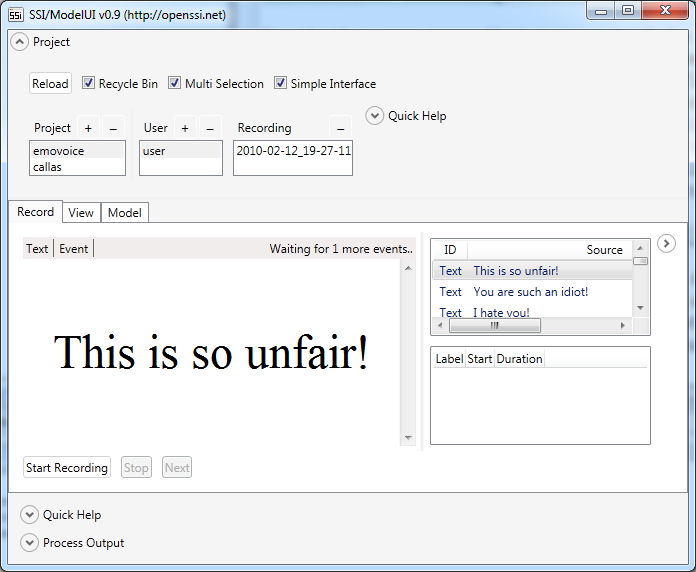
\includegraphics[scale=0.5]{pics/record_gui.png}
\end{center}
\vspace{-0.5cm}
\caption{The record panel.}
\label{fig:record_gui}
\end{figure}

The record panel consists of a web browser to display the stimuli slides. If no recording is running the user can browse through the stimuli slides in the upper list on the right. If a slide is selected its content is displayed in the web browser. A status bar above the web browser gives additional information about the type of source and the kind of trigger connected to the slide (see Section \ref{lab:project_create}). During a recording events triggered by the pipeline are collected in the lower list on the right.

\section{New Recording}\label{lab:project_new}

To start a new recording a user must be selected (if multiple user names are selected the first user in the list will be taken). A new recording is started by clicking on the \texttt{'Start Recording'} button below the web browser. As soon as the pipeline starts to record(which may take a couple of seconds) the first slide will be displayed. While the user follows the instructions on the screen the pipeline continues to capture data and if an event (e.g. a utterance) is detected it will be displayed in the event list. Sometimes a certain number of events must be detected before the next slide is displayed. In other cases a countdown is used or the user is asked to press the \texttt{'Next'} button below the browser. The recording stops automatically when the last stimuli slide has been shown or the user presses the \texttt{'Stop'} button. Now, the pipeline will be stopped (which may again take a couple of seconds) and the recording is stored for the current user.

